\chapter{Demostración de búsqueda con el algoritmo de Grover}
\label{ch:demostracion}

Este capítulo desarrolla un único programa Qalc\footnote{Código fuente disponible en \url{https://github.com/Guillex387/qalc}.} de principio a fin, \lstinline|examples/grover_2bit.qalc|, que ejercita en conjunto todas las fases descritas en los capítulos anteriores, el sistema de tipos lineal del \autoref{ch:analisis-semantico}, el aplanador y la comprobación de consumo lineal del \autoref{ch:backend}, y la generación de código hacia OpenQASM~3 de la \autoref{sec:codegen}, sobre un caso concreto y completo en vez de fragmentos aislados. El programa implementa una búsqueda con el algoritmo de Grover sobre un espacio de 2 cúbits, y usa exclusivamente características del lenguaje ya implementadas a fecha de este capítulo.

\section{Planteamiento del problema de búsqueda}
\label{sec:grover-problema}

El espacio de búsqueda es el conjunto $\{0, 1, 2, 3\}$, representado sobre un registro de 2 cúbits. La condición que marca la solución es $a + 1 = 3$, que tiene una única solución, $a = 2$. El algoritmo de Grover amplifica la amplitud del estado marcado aplicando repetidamente un oráculo que invierte su fase seguido de un difusor que invierte las amplitudes en torno a la media; el número óptimo de iteraciones es, aproximadamente, $\frac{\pi}{4}\sqrt{N/M}$, donde $N$ es el tamaño del espacio de búsqueda y $M$ el número de soluciones marcadas. Para $N = 4$ y $M = 1$ ese número es exactamente $1$, así que una única iteración basta para maximizar la probabilidad de medir el estado solución.

Expresar esta búsqueda exige, en primer lugar, aritmética cuántica reversible (una suma y una comparación de igualdad sobre registros de 2 bits) para poder describir la condición $a + 1 = 3$ como un circuito, y en segundo lugar los mecanismos de composición funcional y de iteración genérica ya presentados en capítulos anteriores para expresar el oráculo, el difusor y el bucle de Grover como funciones ordinarias del lenguaje.

\section{Aritmética reversible}
\label{sec:grover-sumador}

La suma de dos registros \lstinline|qu8| se implementa como una función Qalc ordinaria, \lstinline|`+`|, siguiendo el patrón de un sumador de acarreo en cadena (\textit{ripple-carry}) de 2 bits.

\begin{lstlisting}[language={}, caption=Firma y preparación de recursos del sumador ripple-carry]
`+` :: qu8 -> qu8 -> (qu8, qu8, qu8)
`+` a b = linear {
  ac = qcircOfQu8 a,
  bc = qcircOfQu8 b,
  sc = qcircOfQu8 (qu8 0u8),
  c0 = qcircOfQbool (qbool 0i32),
  c1 = qcircOfQbool (qbool 0i32),
  ...
\end{lstlisting}

El bloque \lstinline|linear| convierte los dos sumandos a \lstinline|qcirc| para poder aplicarles puertas de bajo nivel, y construye tres recursos auxiliares nuevos, el registro de suma \lstinline|sc|, inicializado a cero, y dos acarreos de un cúbit, \lstinline|c0| y \lstinline|c1|. El bit 0 de la suma no tiene acarreo de entrada, así que se calcula con dos \lstinline|crossControlled| (el XOR de \lstinline|ac|/\lstinline|bc| sobre \lstinline|sc|) y un \lstinline|crossToffoli| que produce el acarreo \lstinline|c0|. El bit 1 sí arrastra ese acarreo, así que repite el mismo patrón incorporando \lstinline|c0| como un tercer sumando, y produce un segundo acarreo, \lstinline|c1|, que representaría el desbordamiento de la suma de 2 bits. Como el problema de búsqueda no necesita ese desbordamiento, ambos acarreos se descomputan con \lstinline|uncomputeQbool| antes de devolver el resultado, liberando esos dos cúbits auxiliares. El resultado final es la tupla \lstinline|(ac, bc, sc)|, es decir, los dos sumandos, que la operación no consume, y la suma.

\section{Comparador y kickback de fase}
\label{sec:grover-comparador}

Comparar dos registros \lstinline|qu8| por igualdad, \lstinline|`==`|, sigue una estrategia distinta a la del sumador, ya que su resultado no es un registro nuevo sino un único cúbit de fase que marca las soluciones sin necesidad de medirlas.

\begin{lstlisting}[language={}, caption=Preparación del ancilla de fase del comparador de igualdad]
`==` :: qu8 -> qu8 -> (qu8, qu8, qbool)
`==` sum target = linear {
  sc = qcircOfQu8 sum,
  tc = qcircOfQu8 target,
  rc = qcircOfQbool (qbool 0i32) |> X |> H,
  ...
\end{lstlisting}

El cúbit \lstinline|rc| se prepara en el estado aplicando \lstinline|X| y luego \lstinline|H| sobre un \lstinline|qbool| recién construido a cero; es la preparación estándar para el truco de \textit{kickback} de fase, en la que una puerta controlada sobre un objetivo e imprime una fase $-1$ sobre el estado de control en vez de modificar el objetivo. El registro \lstinline|target| se reutiliza como memoria temporal, ya que sus cúbits se convierten en indicadores de coincidencia bit a bit con parejas \lstinline|crossControlled|/\lstinline|X|, un Toffoli cruzado los combina en el ancilla de fase, y las mismas operaciones se repiten en orden inverso para devolver \lstinline|target| a su valor original antes de devolverlo, sin dejar ningún cúbit auxiliar adicional pendiente de descomputar.

\section{Oráculo y difusor}
\label{sec:grover-oraculo}

El oráculo compone las dos operaciones anteriores para marcar los estados del registro de búsqueda que satisfacen $a + b_\text{const} = \text{target}_\text{const}$, donde las dos constantes llegan como parámetros clásicos de la propia función.

\begin{lstlisting}[language={}, caption=Oráculo que compone la suma y la comparación de igualdad]
oracle :: u8 -> u8 -> qcirc -> qcirc
oracle bConst targetConst c = linear {
  a = qu8OfQcirc c,
  b = qu8 bConst,
  target = qu8 targetConst,
  (a, b, sum) = a + b,
  (sum, target, isMatch) = sum == target,
  uncomputeQbool isMatch,
  uncomputeQu8 target,
  uncomputeQu8 sum,
  uncomputeQu8 b,
  return qcircOfQu8 a
};
\end{lstlisting}

Tras marcar la fase con \lstinline|isMatch|, el oráculo descomputa en orden inverso absolutamente todo lo que construyó (el propio \lstinline|isMatch|, el registro \lstinline|target|, la suma y la constante \lstinline|b|), de modo que lo único que sobrevive a la función es el registro de búsqueda original, ahora con la fase de sus estados solución invertida. El difusor, por su parte, es la secuencia estándar de Grover sobre el registro completo, sin necesidad de ningún recurso auxiliar.

\begin{lstlisting}[language={}, caption=Difusor de Grover sobre el registro de búsqueda]
diffuser :: qcirc -> qcirc
diffuser c = c |> H |> X |> controlled 0 1 Z |> X |> H;
\end{lstlisting}

\section{Punto de entrada y despliegue con repeat}
\label{sec:grover-main}

\lstinline|grover| encadena el oráculo y el difusor mediante el built-in \lstinline|repeat| introducido en el \autoref{sec:repeat}, recibiendo el número de iteraciones y el propio oráculo como parámetros de orden superior.

\begin{lstlisting}[language={}, caption=Iteración de Grover parametrizada por el número de rondas y el oráculo]
grover :: i32 -> (qcirc -> qcirc) -> qcirc -> qcirc
grover n oracleFn c = repeat n ((c) -> c |> oracleFn |> diffuser) c;

main :: qio<u8>
main =
  qcirc 2i32 |> H |> grover 1i32 ((c) -> oracle 1u8 3u8 c) |> measure;
\end{lstlisting}

Las constantes del oráculo, \lstinline|1u8| y \lstinline|3u8|, deben conocerse en tiempo de compilación, ya que fijan las puertas \lstinline|X| que inicializan los registros \lstinline|qu8| correspondientes (\autoref{sec:entry-point}); por eso \lstinline|main| no toma ningún parámetro clásico en este programa, a diferencia de un circuito que reciba, por ejemplo, un ángulo de rotación en tiempo de ejecución. La única iteración de Grover que exige el \autoref{sec:grover-problema} se pasa igualmente como constante al invocar \lstinline|grover|, y es \lstinline|eval_repeat| (\autoref{sec:repeat}) quien la despliega en tiempo de compilación, sustituyendo la lambda \lstinline|(c) -> c |> oracleFn |> diffuser| por una única aplicación directa de \lstinline|oracle| seguida de \lstinline|diffuser|.

\section{Resultado de la compilación}
\label{sec:grover-resultado}

Compilar este programa reserva siete registros cuánticos.

\begin{itemize}
  \item \lstinline|q0| es el registro de búsqueda de 2 cúbits sobre el que actúan el oráculo y el difusor.
  \item \lstinline|q1| y \lstinline|q2| son las constantes \lstinline|bConst|/\lstinline|targetConst| del oráculo, construidas con las puertas \lstinline|X| que fijan su valor.
  \item \lstinline|q3| es la suma intermedia del sumador.
  \item \lstinline|q4| y \lstinline|q5| son los dos acarreos del sumador, descomputados antes de terminar la función.
  \item \lstinline|q6| es el ancilla de fase del comparador de igualdad.
\end{itemize}

El siguiente fragmento corresponde al sumador ripple-carry sobre esos registros, cruzando \lstinline|q0|/\lstinline|q1| hacia \lstinline|q3| con la ayuda de los acarreos \lstinline|q4|/\lstinline|q5|.

\begin{lstlisting}[language={}, caption=Fragmento del sumador ripple-carry en el OpenQASM 3 emitido]
cx q0[0], q3[0];
cx q1[0], q3[0];
ccx q0[0], q1[0], q4[0];
cx q0[1], q3[1];
cx q1[1], q3[1];
cx q4[0], q3[1];
\end{lstlisting}

El listado completo, incluyendo la preparación de constantes, el comparador de igualdad, la descomputación de cada recurso auxiliar y el difusor final, se recoge en el \autoref{ch:grover-qasm}. La \autoref{fig:grover-circuito} muestra el diagrama de circuito correspondiente, generado a partir de ese mismo texto OpenQASM~3 con \lstinline|scripts/render_qasm.py|, un script que carga el circuito con \lstinline|qiskit.qasm3.loads| y lo dibuja con Qiskit.

\begin{figure}[H]
  \centering
  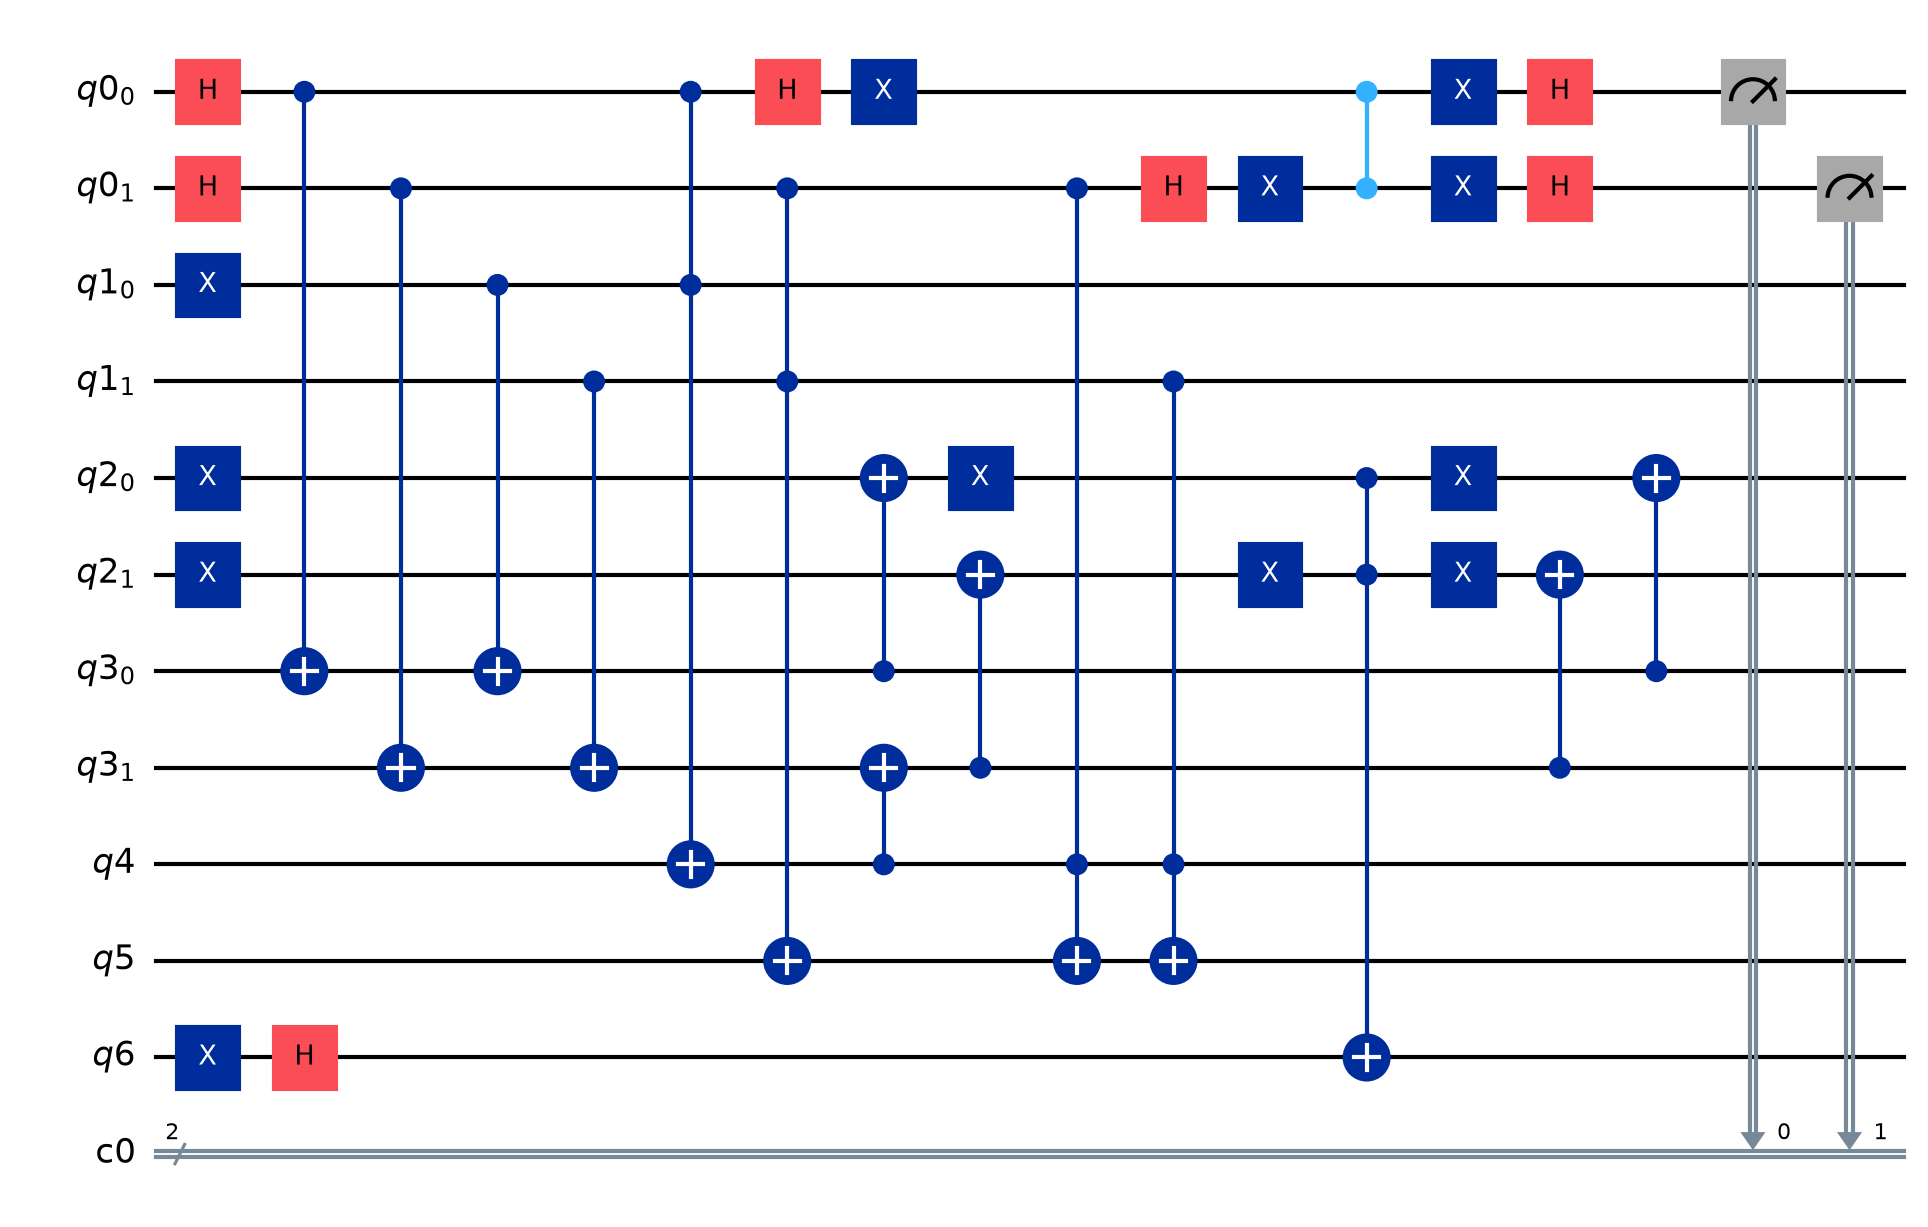
\includegraphics[width=\textwidth]{images/grover_2bit_circuit}
  \caption{Circuito generado para la demostración de búsqueda de Grover}
  \label{fig:grover-circuito}
\end{figure}

Las líneas de comentario \lstinline|// uncompute qN| que aparecen en el listado señalan dónde el comprobador de consumo lineal ya ha verificado que ese registro se libera correctamente, ya que \lstinline|uncompute| es en sí mismo una operación de solo efecto que no emite ninguna puerta.

\section{Hacia una biblioteca estándar de funciones cuánticas}
\label{sec:grover-stdlib}

Ninguna de las funciones de este capítulo, \lstinline|`+`|, \lstinline|`==`|, \lstinline|oracle|, \lstinline|diffuser| ni \lstinline|grover|, es un built-in del compilador. Todas están escritas en Qalc ordinario, en el propio fichero del ejemplo, apoyándose únicamente en el pequeño núcleo de built-ins ya presentado en capítulos anteriores, las puertas cuánticas básicas, \lstinline|crossControlled|/\lstinline|crossToffoli| para cruzar registros, \lstinline|repeat| para la iteración genérica, y las conversiones de identidad entre \lstinline|qcirc| y los tipos de alto nivel. Esto demuestra que esa superficie de built-ins ya es suficiente para construir, con las herramientas ordinarias del lenguaje, componentes reutilizables de un nivel de abstracción considerablemente más alto que una puerta individual.

El prototipo actual, sin embargo, obliga a redefinir estas funciones en cada programa que las necesite, ya que no existe todavía ninguna biblioteca de funciones compartida entre programas Qalc distintos. La línea futura \textit{Ampliación de la librería estándar de tipos y operaciones}, ya identificada en el \autoref{ch:conclusiones}, encuentra en \lstinline|`+`|, \lstinline|`==`|, \lstinline|diffuser| y \lstinline|grover| un punto de partida concreto, ya que son exactamente el tipo de operación reutilizable (aritmética modular sobre registros de tamaño fijo y bloques estándar de algoritmos de búsqueda) que una biblioteca estándar debería distribuir junto con el compilador en vez de dejar que cada programa las reimplemente desde cero.
